%\documentclass[12pt,a4paper]{report}
\documentclass[DIV=calc,paper=a4,fontsize=11pt,openany]{book}
\usepackage[utf8]{inputenc}
\usepackage[spanish]{babel}
\renewcommand{\baselinestretch}{1.3}
\usepackage[autostyle,spanish=mexican]{csquotes}
\MakeOuterQuote{"}
\usepackage{amsmath,amsfonts,amsthm,amssymb,wasysym}
\usepackage{graphicx}
\usepackage{amsmath}
\usepackage{amsfonts}
\usepackage{latexsym}
\usepackage{enumerate}
\usepackage{amssymb}
\usepackage{makeidx}
\usepackage{tikz}
\usepackage{pstricks} 
\usepackage{cancel}
\usepackage{caption}
\usepackage{float} %flotador de label
\usepackage{wrapfig} %Permite figuras o tablas que tienen texto
\usepackage{shadow}
\usepackage{fancyhdr} %definir pie de pagina y encabesados
\usepackage{multicol}
\usepackage[all]{xy}
\usepackage{underoverlap}
\usepackage{asymptote}
\usepackage{environ}
\usepackage{multicol}
\usepgflibrary{shapes.misc}
\usepackage{MnSymbol}
\usepackage{mathrsfs}
\usepackage[left=3cm,right=3.7cm,top=2.8cm,bottom=2.7cm]{geometry}
\usepackage{pdfpages}
\usepackage[colorinlistoftodos, textwidth=3cm, shadow]{todonotes}
 \definecolor{verdeoscuro}{RGB}{6,18,97}
 
%%%encabezado y pie de pagina1
\renewcommand{\footrulewidth}{2pt}  %regla de pie de pagina
\pagestyle{fancy} %para que aparescaa regla orizontal
\columnseprule=1.2pt %regla de columna
\columnsep=25pt  %espacio en blando de la columna y texto
%encabezado

\lhead[{\vspace*{-0.2cm}\red ESTADISTICA II} ] {\bf\red UNIVERSIDAD NACIONAL DE SAN CRISTÓBAL DE HUAMANGA\ -\ ING. DE SISTEMAS }
\chead[]{}
\rhead[\rightmark]{\bf \blue }

%pie de pagina
\definecolor{blue(pigment)}{RGB}{20,70,60}
\lfoot[]{\bf }
\cfoot[]{}
\rfoot[]{\vspace*{-0.8cm}\fcolorbox{black}{white}{\Large\bfseries\color{blue(pigment)} {\thepage}}}
\usetikzlibrary{shadows}                          
\newcommand{\preg}[1]{
   \par\vspace{0.6em}\noindent 
                           
\begin{tikzpicture}[baseline=(X.base)]\node       
	[drop shadow,fill=black,draw,very thin] (X) {\color{white} \textsf{\textbf{#1}}}; 
\end{tikzpicture}\hspace{0.4cm}}
 
%sombra%                         
\newcommand{\sombra}[1]{                          
\begin{tikzpicture}[baseline=(X.base)]\node       
	[drop shadow,fill=white,draw,very thin] (X) {#1}; 
\end{tikzpicture}}

%ejercicios%
\newcommand{\Ejercicio}[1]{   
\begin{tikzpicture}
	\node[rounded rectangle, white, fill=black!70, draw]
	{\sf {Ejercicio} {\normalsize  #1}};
\end{tikzpicture}
}
\renewcommand{\thesection}{\arabic{section}}
%%%%%%%contador%%%%%%%%
\newcounter{contador}[section] 
\setcounter{contador}{0}       

%%%%%%%%definimos ambiente pregunta y solucion%%%%%%%%%%%%
\usepackage{colortbl}                                                                               
\definecolor{col}{RGB}{45,07,107}

%solucion%                    
\newcommand\sol{\noindent                                         
 \\[0.4em]
  { \slshape \color{red}\textbf{Resolución}}
  \\[0.3em]\noindent  }
                     
\makeatother
                                
%%%%comandos particulares%%%%
\newcommand{\af}{\alpha}
\newcommand{\D}{\pmb{D}}
\newcommand{\be}{\beta}
\newcommand{\te}{\theta}
\newcommand{\al}{\displaystyle}
\newcommand{\med}{\scriptstyle}
\newcommand{\imp}{\Rightarrow}
\newcommand{\impp}{\Longleftrightarrow}
\newcommand{\im}{\rightarrow}
\newcommand{\p}{\cdot}
\newcommand{\ca}{\cancel}
\newcommand{\tri}{\therefore}
\newcommand{\sen}{\mathop{\rm sen}\nolimits}
\newcommand{\tg}{\mathop{\rm tg}\nolimits}\newcommand{\ct}{\mathop{\rm ctg}\nolimits}
\newcommand{\R}{\mathbb{R}}
\newcommand{\Z}{\mathbb{Z}}
\newcommand{\N}{\mathbb{N}}
\newcommand{\se}{\overline}
\newcommand{\ang}{\measuredangle}
\newcommand{\an}{\angle}
\newcommand{\tr}{\triangle}
\newcommand{\g}{^\circ}
\newcommand{\spa}{\smallskip}
\newcommand{\spac}{\medskip}
\newcommand{\brazo}{\underbrace}
\newcommand{\medi}{\mbox{m}\measuredangle}
\newcommand{\f}{\frac}
\newcommand{\dist}{\vspace{-0.5cm}}
\newcommand{\rad}{\;\mbox{rad}}\newcommand{\bi}{\bullet\;\;}
\newcommand{\Del}[1]{\left[#1\right]}
\newcommand{\del}[1]{\left(#1\right)}
\newcommand{\sect}[1]{\leftslice\scriptscriptstyle{#1}}
\newcommand{\q}{\sqrt}
\newcommand{\y}{\;\wedge\;}
\newcommand{\oo}{\;\vee \;}
\newcommand{\sii}{\;\Leftrightarrow\;}
\newcommand{\pt}{\times}
\newcommand{\s}{\sec\mathsf{h}}
\newcommand{\ta }{\tan\mathsf{h}}
\newcommand{\limt}{\lim_{n\rightarrow \infty}}
\newcommand{\prt}{\partial}
\newcommand{\M}{\geq}
\newcommand{\m}{\leq}
\newcommand{\vol}{\mathrm{Vol}}
\newcommand{\area}{\mathrm{Area}}
\newcommand{\yy}{\overline{y}}
\newcommand{\vx}{\overline{x}}
\newcommand{\hs}{\hspace{0.6cm}}
\newcommand{\dd}{\mathrm{d}}
\newcommand{\n}{\nabla}
\usepackage{amsmath}
\usepackage{graphicx,tcolorbox}
\definecolor{blue(pigment)}{RGB}{20,70,60}
\definecolor{som}{RGB}{68,05,5}
\usetikzlibrary{shadows} 

%---------RTA----------%
\newcommand{\ptas}[1]{
\begin{flushright}
	\begin{tikzpicture}
	\node[rounded rectangle, white, fill=black!70, draw]
	{\sf {clave} {\normalsize #1}};
	\end{tikzpicture}
\end{flushright}}
% Estilos: Sonny, Lenny, Glenn, Conny, Rejne, Bjarne, Bjornstrup
\usepackage[Sonny]{fncychap}


\begin{document}%INICIO DEL DOCUMENTO 


\Ejercicio{10}\\

El tiempo de vida de una bateria es una variable aleatoria \textit{X} con distribución exponencial de parámetro: $1/\theta$. Se escoge una muestra de n baterías\\
a) Halle el error estandar de la media muestral $\overline{X}$\\
b) Si la muestra aleatoria es de tamaño $ n = 64 $, ¿con que probabilidad diferirá $\overline{X}$ del verdadero valor $\theta$ en menos de un error estándar?\\
c) ¿Qué tamaño de muestra mínimo sería necesario para que la media muestral $\overline{X}$ tenga un error estándar menor a un $5\%$ del valor real de $\theta?$\\
d) Asumiendo muestra grande, ¿qué tamaño de muestra sería necesario para que $\overline{X}$ difiera de $\theta$ en menos de $10\%$
de $\theta$ con $95\%$ de probabilidad?\\

\textbf{\textit{\textcolor{blue}{Solución:}}}\\

a) 
\begin{center}
$f(x) = \dfrac{1}{\theta}e^{\frac{-x}{\theta}}$ ; $x\geqslant 0$
\end{center}
\begin{center}
$\sqrt{Var(\overline{X})} = \dfrac{\theta}{\sqrt{n}}$ \  error estandar
\end{center}
\begin{center}
$Var(\overline{X}) = \dfrac{\theta^{2}}{n}$
\end{center}
\[ E(x) = u = \int_{0}^{+\infty} \! \dfrac{x}{e}e^\frac{-x}{\theta} \, dx 
\]
\[\gamma(\alpha)=\int_{0}^{+\infty} \! y^{\alpha-1}e^{-y} \, dy\]
\begin{center}
$(\alpha-1)!$ \ ; $ \alpha \in N $
\end{center}
\begin{center}
$\gamma(\alpha) = (\alpha-1)!\gamma(\alpha-1)$ ; para $\alpha \neq N$
\end{center}
\[ E(x) = u = \theta\int_{0}^{+\infty} \! (\dfrac{x}{\theta})^{2-1}e^\frac{-x}{\theta} \, d(\frac{x}{\theta})
\]
\begin{center}
$\gamma(2)=(2-1)! = 1$
\end{center}
\begin{center}
$ E(x)= \theta $
\end{center}
\[ E(x^{2})  \theta^{2}\int_{0}^{+\infty} \! (\dfrac{x}{\theta})^{3-1}e^\frac{-x}{\theta} \, d(\frac{x}{\theta})
\]
\begin{center}
$E(x^{2})=2\theta^{2}$
\end{center}
\begin{center}
$\gamma(3)= 2!= 2$
\end{center}
\begin{center}
\colorbox{yellow}{$\sigma^{2} = Var(x) = 2\theta^{2}-\theta^{2} = \theta^{2}$}
\end{center}
\newpage
b) Teorema Central de Limite\\
\begin{center}
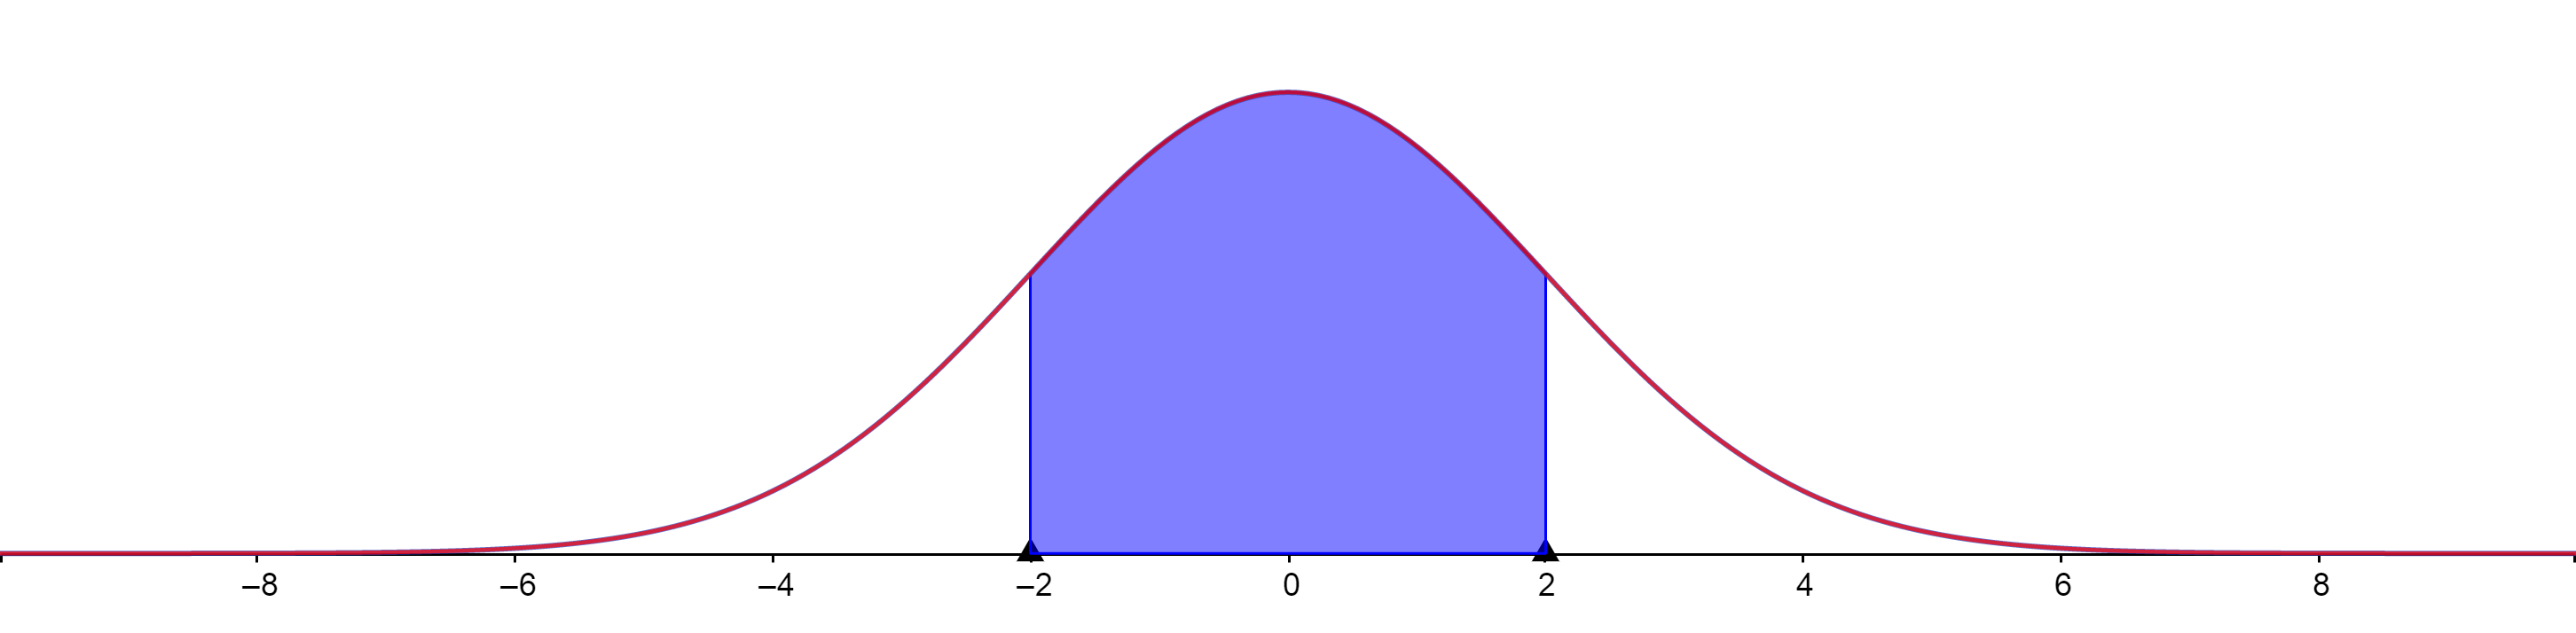
\includegraphics[scale=0.15]{Imagenes/geogebra-export.png} 
\end{center}
\begin{center}
$P(\mid\overline{X}- \sigma \mid \leq \dfrac{\theta}{\sqrt{n}} \cong 0.68$
\end{center}
\begin{center}
$P(-\theta \leq x-4\leq \theta)$
\end{center}
\begin{center}
$P(\mid x - u \mid \leq 2\theta) \cong 0.9544$
\end{center}
\begin{center}
$P(\mid x - u \mid \leq 3\theta) \cong 0.99$
\end{center}
\begin{center}
$u\overline{X} = u = \theta$
\end{center}
\begin{center}
$Var(\overline{X}) = \theta^{2}x = \theta^{2}$
\end{center}
\begin{center}
$  P(\mid \overline{X} - \theta \mid \leq \dfrac{\theta}{\sqrt{n}})$
\end{center}

\begin{center}
$P( \overline{X} - \theta  \leq \dfrac{\theta}{8}) = P\left( \dfrac{\overline{X}- \theta}{\frac{\theta}{8}} \leq \dfrac{\frac{\theta}{8}}{\frac{\theta}{8}}\right)$ 
\end{center}
\begin{center}
$ P( \overline{X} - \theta  \leq \dfrac{\theta}{8}) = P(z \leq 1$
\end{center}
\begin{center}
\colorbox{yellow}{$P( \overline{X} - \theta  \leq \dfrac{\theta}{8}) = 0,68$} 
\end{center}
c)
\begin{center}
$\dfrac{\theta}{\sqrt{n}} < 0.050\theta \Rightarrow \dfrac{1}{\sqrt{n} < 0,05}$
\end{center}
\begin{center}
$1\dfrac{1}{0.05}<\sqrt{n} \Rightarrow 20^{2} < \sqrt{n}^{2}$
\end{center}
\begin{center}
\colorbox{yellow}{$20 < \sqrt{n} \Rightarrow 400 < n$}
\end{center}
d)
\begin{center}
$P(\mid \overline{X}-u \mid < 0.1\theta)=0.95$
\end{center}
\begin{center}
$P\left( \dfrac{\overline{X}-u}{\frac{\sigma}{\sqrt{n}}} < \dfrac{0.1\theta}{\frac{\sigma}{\sqrt{n}}}\right)= 0.95$
\end{center}
\begin{center}
$P(\mid Z \mid < 0.1\sqrt{n}) = 0.95$
\end{center}
\begin{center}
$P(-0.1\sqrt{n} < z < 0.1\sqrt{n}) = 0.95$
\end{center}
\begin{center}
$P(z < 0.1\sqrt{n})- (1-P(z < 0.1\sqrt{n}) = 0.95$
\end{center}
\begin{center}
$2P( z < 0.1\sqrt{n}) = 1.95$
\end{center}
\begin{center}
$P(z < 0.1\sqrt{n}) = 0.975$
\end{center}
\begin{center}
$0.1\sqrt{n} = 1.96$
\end{center}
\begin{center}
$\sqrt{n} = 19.6$
\end{center}
\begin{center}
\colorbox{yellow}{$n = 385 $}
\end{center}











\end{document}%FINAL DEL DOCUMENTO%
